\subsection{$ E2 $ transitions of the oxygen isotopes}
Here we will only investigate the $E2$ between the first $2^+$ and the first $0^+$, i.e. $B(E2; 2_1^+ \rightarrow 0_1^+)$, using the USDA, USDB and CCEI interactions, given in Fig. \ref{oxygen-be2}. For the experimental data there are only three values, however it is notable that they become closer to the theoretical values as neutrons are added, with the largest discrepancy occurring for the $^{18}$O isotope. The reason might be due to the fact we are neglecting $p$-shell core-excitations when using only the $sd$-shel model space. It was found in \cite{Lawson1976} that the $0_2^+$ should have a dominant $4p-2h$ component. However there are indications that mixing should arise, and perhaps with the $0_1^+$. As for the $2^+_1$, there might be less mixing with an intruder configuration since the $2^+_3$, which has a large intruder component, is high in energy (5.255 MeV) 	 and thus mixes less with the $2^+_1$. The problem for mixing of these states due to the truncation in the $np–mh$ sequence is discussed in \cite{Warburton1992a}. Therefore, when close to the $^{16}$O core, e.g. at $^{18}$O, a some part of the $p$-shell is missing in the wave function of $0^+_1$ rendering less components in the wave functions to connect between the $0_1^+$ and the $2_1^+$ and hence yielding a smaller $B(E2)$ value. As neutrons are added to the $^{16} $O core, the $p$-shell core-excitations move to higher energy and mix less with the low-lying states, then the $sd$-shell model space becomes a better approximation. As seen in Fig. \ref{oxygen-be2}, this is correct for all three interactions which operate in the $sd$-shell. Although the CCEI does not reproduce energies as well as USDA and USDB, it gives a slightly better approximation for the $B(E2; 2_1^+ \rightarrow 0_1^+)$. Yet, the differences are minor and other observables should be examined.

\begin{figure}[h]
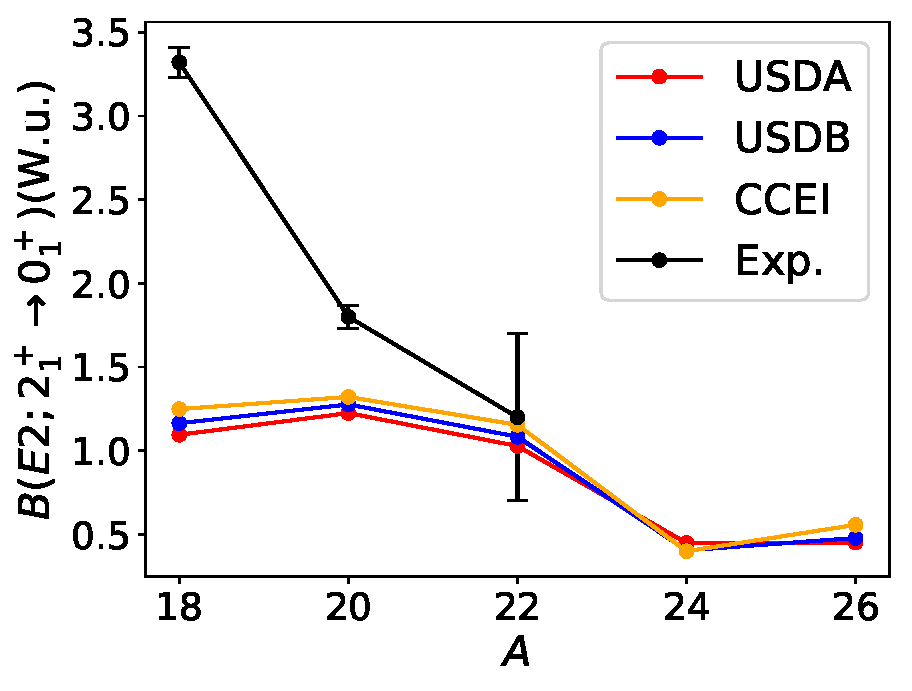
\includegraphics[width=1\linewidth]{../figures/oxygen-be2.pdf}
\caption{$B(E2; 2^+ \rightarrow 0^+)$ of experimental (black), the USDA (red), USDB (blue) and CCEI (orange) interactions for $^{18-26}$O. \label{oxygen-be2}}
\end{figure}


